\documentclass[12pt,a4paper]{jarticle}
%
\topmargin=-5mm
\oddsidemargin=-5mm
\evensidemargin=-5mm
\textheight=235mm
\textwidth=165mm
%
\title{FDPS講習会の手引}
\author{谷川衝、岩澤全規、細野七月、似鳥啓吾、村主崇行、牧野淳一郎}
\date{\today}
%\pagestyle{empty}
\usepackage{graphicx}
\usepackage{wrapfig}
\usepackage{lscape}
\usepackage{amssymb}
\usepackage{amsmath}
\usepackage{bm}
\usepackage{setspace}
%\usepackage{listings,jlisting}
\usepackage{color}
\usepackage{ascmac}
\usepackage{here}
\usepackage[dvipdfmx]{hyperref}
\usepackage{pxjahyper}

\newcommand{\underbold}[1]{\underline{\bf #1}}
\newcommand{\redtext}[1]{\textcolor{red}{#1}}

%\setcounter{secnumdepth}{4}
%%%%%%%%%%%%%%%%%%%%%%%%%%%%%%%%%%
\setcounter{secnumdepth}{5}
\makeatletter
\newcommand{\subsubsubsection}{\@startsection{paragraph}{4}{\z@}%
{1.5\baselineskip \@plus.5\dp0 \@minus.2\dp0}%
{.5\baselineskip \@plus2.3\dp0}%
{\reset@font\normalsize\bfseries}
}
\newcommand{\subsubsubsubsection}{\@startsection{subparagraph}{5}{\z@}%
{1.5\baselineskip \@plus.5\dp0 \@minus.2\dp0}%
{.5\baselineskip \@plus2.3\dp0}%
{\reset@font\normalsize\itshape}
}
\makeatother
\setcounter{tocdepth}{5}
%%%%%%%%%%%%%%%%%%%%%%%%%%%%%%%%%%

\begin{document}
\maketitle
\tableofcontents

\newpage

\section{プログラム}

\begin{itemize}

\item 13:00 -- 14:00 FDPSの講義
  \begin{itemize}
  \item 13:00 -- 13:05 イントロダクション (牧野淳一郎)
  \item 13:05 -- 13:20 概要説明 (谷川衝)
  \item 13:20 -- 13:35 FDPS詳細1 -- APIと内部構造 (岩澤全規)
  \item 13:35 -- 13:50 FDPS詳細2 -- サンプルコード解説 (細野七月)
  \item 13:50 -- 14:00 Q\&A
  \end{itemize}

\item 14:00 -- 15:30 FDPSの実習
  \begin{itemize}
  \item FDPSのインストール
  \item サンプルコードの使用1 (重力N体シミュレーションコード)
  \item サンプルコードの使用2 (SPHシミュレーションコード)
  \end{itemize}

\item 15:30 -- 17:00 FDPS使用に関する相談

\end{itemize}

\newpage

\section{FDPSの実習}

\subsection{環境の設定}

FOCUSの計算機にログインしたら、以下のコマンドを実行する。
\begin{screen}
\begin{verbatim}
$ module load gnu/openmpi165
\end{verbatim}
\end{screen}

\subsection{FDPSの入手}

\begin{itemize}
\item FOCUSの計算機を使用する場合:

  以下のコマンドを実行し、FDPSを自分のカレントディレクトリにコピーする
  (「\verb|$|」はコマンドプロンプトであるので、「\verb|$|」を打ち込む必
  要はない)。
  \begin{screen}
\begin{verbatim}
$ cp -r ~uiud0014/FDPS-master .
\end{verbatim}
  \end{screen}
  以上により、ディレクトリFDPS-masterがコピーされる。

\item FOCUSの計算機以外を使用する場合: 

  https://github.com/FDPS/FDPS からFDPSの最新版をダウンロードし、好きな
  ディレクトリ下で解凍する。これによってディレクトリFDPS-masterが出来る。

\end{itemize}

以下ではディレクトリFDPS-masterがあるディレクトリの名前をfdpsとする。

\subsection{サンプルコードの使用}

本節ではサンプルコードの使用方法について記述する。サンプルコードには重
力$N$体シミュレーションコードと、SPHシミュレーションコードがある。最初
に重力$N$体シミュレーションコード、次にSPHシミュレーションコードの使用
について記述する。ここでの使用方法の説明はFOCUSの計算機を使用する場合に
限る。

\subsubsection{重力$N$体シミュレーションコード}

\subsubsubsection{概要}

以下の手順で本コードを使用できる。
\begin{itemize}
\item ディレクトリfdps/FDPS-master/sample/nbodyに移動
\item makeを実行
\item ジョブの投入
\item 結果の解析
\item OpenMP/MPIの利用(オプション)
\end{itemize}

\subsubsubsection{ディレクトリ移動}

ディレクトリfdps/FDPS-master/sample/nbodyに移動する。

\subsubsubsection{makeの実行}

makeコマンドを実行する。

\subsubsubsection{ジョブの投入}

以下のコマンドを実行し、ジョブの投入を行う。
\begin{screen}
\begin{verbatim}
$ sbatch nbody1.sh
\end{verbatim}
\end{screen}

正しくジョブが投入されている場合、squeueコマンドを実行すると、例えば以
下のようにログが出力される。
\begin{screen}
\begin{verbatim}
 JOBID PARTITION     NAME     USER ST       TIME  NODES NODELIST(REASON)
189090     c006m    nbody uiud0014  R       0:00      1 c017
\end{verbatim}
\end{screen}

ジョブのキャンセルは以下のコマンドで実行できる。
\begin{screen}
\begin{verbatim}
$ scancel JOBID
\end{verbatim}
\end{screen}
JOBIDは上のsqueueコマンドで表示されたJOBIJの番号である(上で言えば、
189090)。

正しくジョブが終了すると、ファイルstdout.logの最後には以下のようなログ
が出力されている。energy errorは絶対値で$1 \times 10^{-3}$のオーダーに
収まっていればよい。
\begin{screen}
\begin{verbatim}
time:  9.5000000 energy error: -3.804653e-03
time:  9.6250000 energy error: -3.971175e-03
time:  9.7500000 energy error: -3.822343e-03
time:  9.8750000 energy error: -3.884310e-03
******** FDPS has successfully finished. ********
\end{verbatim}
\end{screen}

\subsubsubsection{結果の解析}

ディレクトリresultに粒子分布を出力したファイル"000x.dat"ができている。
xは0から9の値で、時刻を表す。出力ファイルフォーマットは1列目から順に粒
子のID, 粒子の質量、位置のx, y, z座標、粒子のx, y, z軸方向の速度である。

ここで実行したのは、粒子数1024個からなる一様球(半径3)のコールドコラプ
スである。コマンドライン上で以下のコマンドを実行すれば、時刻9における
xy平面に射影した粒子分布を見ることができる。
\begin{screen}
\begin{verbatim}
$ gnuplot
$ plot "result/0009.dat" using 3:4
\end{verbatim}
\end{screen}

他の時刻の粒子分布をプロットすると、一様球が次第に収縮し、その後もう一
度膨張する様子を見ることができる(図\ref{fig:nbody}参照)。

\begin{figure}
  \begin{center}
        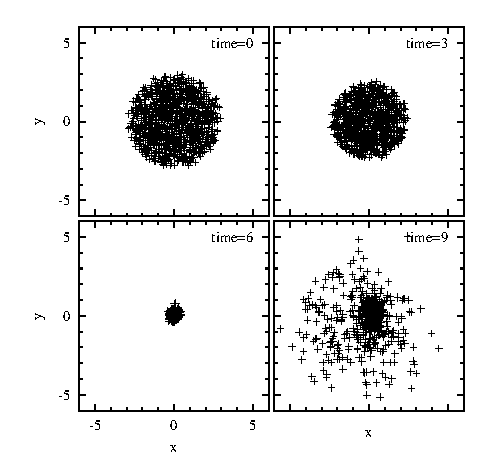
\includegraphics[width=10cm,bb=0 0 220 220]{fig/nbody.eps}
  \end{center}
  \caption{}
  \label{fig:nbody}
\end{figure}

\if 0
粒子数を10000個にして計算を行いたい場合には以下のように実行すればよい
(MPIを使用しない場合)。
\begin{screen}
\begin{verbatim}
$ ./nbody.out -N 10000
\end{verbatim}
\end{screen}
\fi

\subsubsubsection{OpenMP/MPIの利用}

OpenMPやMPIを利用する場合について以下に記述する。
\begin{itemize}
\item OpenMPのみ使用の場合
  \begin{itemize}
  \item Makefileの編集
    \begin{itemize}
    \item マクロCCにOpenMP対応のC++コンパイラを代入する
    \item "CFLAGS += -DPARTICLE\_SIMULATOR\_THREAD\_PARALLEL -fopenmp"の
      行のコメントアウトを外す
    \end{itemize}
  \item makeコマンドを実行する。
  \item 「sbatch nbody2.sh」というコマンドを実行し、ジョブを投入する。
  \item ファイルstdout.log内でスレッド数が4であることを確認できる。
  \end{itemize}

\item MPIのみ使用の場合
  \begin{itemize}
  \item Makefileの編集
    \begin{itemize}
    \item マクロCCにMPIC++コンパイラを代入する
    \item "CFLAGS += -DPARTICLE\_SIMULATOR\_MPI\_PARALLEL"の行のコメント
      アウトを外す
    \end{itemize}
  \item makeコマンドを実行する。
  \item 「sbatch nbody3.sh」というコマンドを実行し、ジョブを投入する。
  \item ファイルstdout.log内でプロセス数が2であることを確認できる。
  \end{itemize}

\item OpenMPとMPIの同時使用の場合
  \begin{itemize}
  \item Makefileの編集
    \begin{itemize}
    \item マクロCCにMPI対応のC++コンパイラを代入する
    \item "CFLAGS += -DPARTICLE\_SIMULATOR\_THREAD\_PARALLEL -fopenmp"の
      行のコメントアウトを外す(インテルコンパイラの場合は-fopenmpを外す)
    \item "CFLAGS += -DPARTICLE\_SIMULATOR\_MPI\_PARALLEL"の行のコメント
      アウトを外す
    \end{itemize}
  \item makeコマンドを実行する。
  \item 「sbatch nbody4.sh」というコマンドを実行し、ジョブを投入する。
  \item ファイルstdout.log内でプロセス数が2、スレッド数が4であることを
    確認できる。
  \end{itemize}

\end{itemize}

\if 0
\subsubsubsection{x86版Phantom-GRAPEを使う場合}

まず、使用環境を確認する。Intel CPUまたはAMD CPUを搭載したコンピュータ
を使用しているならば、x86版Phantom-GRAPEを使用可能である。FOCUSの計算機
では、使用可能である。

次にディレクトリ
fdps/FDPS-master/src/phantom\_grape\_x86/G5/newton/libpg5に移動して、ファ
イルMakefileを編集し、コマンドmakeを実行してPhantom-GRAPE のライブラリ
libpg5.aを作る。FOCUSの計算機を使用している場合は、Makefileを編集する必
要はない。

最後に、ディレクトリfdps/FDPS-master/sample/nbodyに戻り、ファイル
Makefile内の\\''\#use\_phantom\_grape\_x86 = yes''の''\#''を消す。make
をしてコンパイルする(OpenMP, MPIの使用・不使用どちらにも対応)と、x86版
Phantom-GRAPEを使用したコードができている。上と同様の方法で実行・結果の
確認を行うとさきほどと同様の結果が得られる。

Intel Core i5-3210M CPU @ 2.50GHz の2コアで性能テスト(OpenMP使用、MPI
不使用)をした結果、粒子数8192の場合に、Phatom-GRAPEを使うと、使わない
場合に比べて、最大で5倍弱ほど高速なコードとなる。以下が最適化された実
行例。
\begin{screen}
\begin{verbatim}
$ ./nbody.out -N 8192 -n 256
\end{verbatim}
\end{screen}
\fi

\subsubsection{SPHシミュレーションコード}

\subsubsubsection{概要}

以下の手順で本コードを使用できる。
\begin{itemize}
\item ディレクトリfdps/FDPS-master/sample/sphに移動
\item makeを実行
\item ジョブの投入
\item 結果の解析
\item OpenMP/MPIの利用(オプション)
\end{itemize}

\subsubsubsection{ディレクトリ移動}

ディレクトリfdps/FDPS-master/sample/sphに移動に移動する。

\subsubsubsection{makeの実行}

makeコマンドを実行する。

\subsubsubsection{ジョブの投入}

以下のコマンドを実行し、ジョブの投入を行う。
\begin{screen}
\begin{verbatim}
$ sbatch sph1.sh
\end{verbatim}
\end{screen}

正しくジョブが投入されている場合、squeueコマンドを実行すると、例えば以
下のようにログが出力される。
\begin{screen}
\begin{verbatim}
 JOBID PARTITION     NAME     USER ST       TIME  NODES NODELIST(REASON)
189090     c006m      sph uiud0014  R       0:00      1 c017
\end{verbatim}
\end{screen}

ジョブのキャンセルは以下のコマンドで実行できる。
\begin{screen}
\begin{verbatim}
$ scancel JOBID
\end{verbatim}
\end{screen}
JOBIDは上のsqueueコマンドで表示されたJOBID番号である(上で言えば、
189090)。

正しくジョブが終了すると、ファイルstdout.logの最後には以下のようなログ
が出力されている。
\begin{screen}
\begin{verbatim}
******** FDPS has successfully finished. ********
\end{verbatim}
\end{screen}

\subsubsubsection{結果の解析}

ディレクトリresultにファイルが出力されている。ファイル名は"00xx.dat"(x
には数字が入る)となっている。ファイル名は時刻を表す。出力ファイルフォー
マットは1列目から順に粒子のID、粒子の質量、位置のx, y, z 座標、粒子の
x, y, z軸方向の速度、密度、内部エネルギー、圧力である。

これは3次元の衝撃波管問題である。以下のコマンドを実行すれば、横軸に粒
子のx座標、縦軸に粒子の密度をプロットできる(時刻は40)。
\begin{screen}
\begin{verbatim}
$ gnuplot
$ plot "result/0040.dat" using 3:9
\end{verbatim}
\end{screen}
正しい答が得られれば、図\ref{fig:sph}のような図を描ける。

\begin{figure}
  \begin{center}
    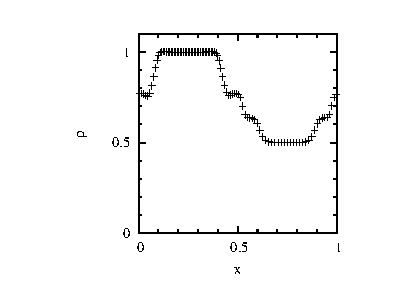
\includegraphics[width=8cm,bb=0 0 150 150]{fig/sph.eps}
  \end{center}
  \caption{}
  \label{fig:sph}
\end{figure}

\subsubsubsection{OpenMP/MPIの利用}

OpenMPやMPIを利用する場合を以下に示す。
\begin{itemize}
\item OpenMPのみ使用の場合
  \begin{itemize}
  \item Makefileの編集
    \begin{itemize}
    \item マクロCCにOpenMP対応のC++コンパイラを代入する
    \item "CFLAGS += -DPARTICLE\_SIMULATOR\_THREAD\_PARALLEL -fopenmp"の
      行のコメントアウトを外す
    \end{itemize}
  \item makeコマンドを実行する。
  \item 「sbatch sph2.sh」というコマンドを実行し、ジョブを投入する。
  \item ファイルstdout.log内でスレッド数が4であることを確認できる。
  \end{itemize}

\item MPIのみ使用の場合
  \begin{itemize}
  \item Makefileの編集
    \begin{itemize}
    \item マクロCCにMPIC++コンパイラを代入する
    \item "CFLAGS += -DPARTICLE\_SIMULATOR\_MPI\_PARALLEL"の行のコメント
      アウトを外す
    \end{itemize}
  \item makeコマンドを実行する。
  \item 「sbatch sph3.sh」というコマンドを実行し、ジョブを投入する。
  \item ファイルstdout.log内でプロセス数が2であることを確認できる。
  \end{itemize}

\item OpenMPとMPIの同時使用の場合
  \begin{itemize}
  \item Makefileの編集
    \begin{itemize}
    \item マクロCCにMPI対応のC++コンパイラを代入する
    \item "CFLAGS += -DPARTICLE\_SIMULATOR\_THREAD\_PARALLEL -fopenmp"の
      行のコメントアウトを外す(インテルコンパイラの場合は-fopenmpを外す)
    \item "CFLAGS += -DPARTICLE\_SIMULATOR\_MPI\_PARALLEL"の行のコメント
      アウトを外す
    \end{itemize}
  \item makeコマンドを実行する。
  \item 「sbatch sph4.sh」というコマンドを実行し、ジョブを投入する。
  \item ファイルstdout.log内でプロセス数が2、スレッド数が4であることを
    確認できる。
  \end{itemize}

\end{itemize}

\end{document}
